\documentclass{beamer}
\usepackage[utf8]{inputenc}

\usepackage{semantic}
\usepackage{graphicx}
\usepackage{booktabs}
\usepackage{todonotes}
\presetkeys{todonotes}{inline}{}

\usepackage[absolute,overlay]{textpos}
% This is to get textpos to play well,
% A stackoverflow user mentioned that this could
% cause problems in some Acrobat Reader versions
% I'll take the chance
\usebackgroundtemplate{}


\mode<presentation> {
\usetheme{boxes} % When headline is wanted use Dresden theme instead
\usecolortheme{seagull}
\setbeamertemplate{footline}[page number]
\setbeamertemplate{navigation symbols}{}
}


%----------------------------------------------------------------------------------------
%	TITLE PAGE
%----------------------------------------------------------------------------------------

\title[APL \& TAIL] % bottom of every slide
  {Teaching kids programming, IT-creativity and modern tech} % title page

\author{\footnotesize{Martin Dybdal} \\ \footnotesize{\texttt{dybber@dybber.dk}}}

\institute {
DIKU \\
University of Copenhagen
}

\date{\footnotesize{Chalmers, 10 October 2015}}

\date{10 November 2015}

\begin{document}

{
\setbeamertemplate{headline}{}
\begin{frame}
  \begin{center}
    
\includegraphics[width=0.7\textwidth]{imagery/codingpirates.png}
  \end{center}
\vspace{-1cm}
\titlepage
\end{frame}
}

%----------------------------------------------------------------------------------------
%	TABLE OF CONTENTS
%----------------------------------------------------------------------------------------

\begin{frame}
\frametitle{Overview}
\tableofcontents
\end{frame}

%----------------------------------------------------------------------------------------
%	CONTENT
%----------------------------------------------------------------------------------------

\section{What is Coding Pirates?}
\begin{frame}
\frametitle{What is Coding Pirates?}
\begin{textblock}{20}(5,5)
 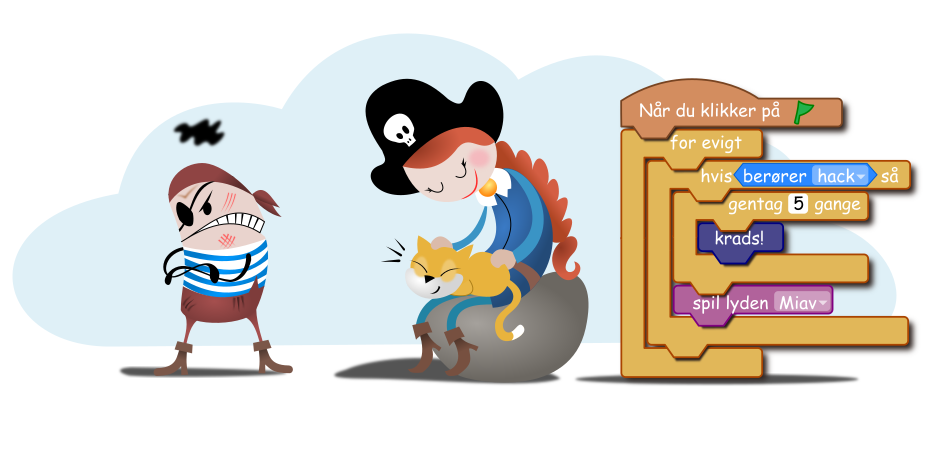
\includegraphics[width=\textwidth]{imagery/cpthack-and-miss1337-transp.png}
\end{textblock}

\begin{itemize}
\item Activity for kids aged 7-17 years
\item A playground - not just two more hours of school
\item An attempt to change the school system
\end{itemize}
\vspace{2cm}
\end{frame}

\subsection{Who are Coding Pirates?}
\begin{frame}
\frametitle{Who are Coding Pirates?}
\begin{itemize}
\item Non-profit organisation
\item +250 volunteers in Coding Pirates network
  \begin{itemize}
  \item Teachers, IT professionals, researchers, librarians, IT students
  \end{itemize}
\item $\sim$700 paying members
\item 24 hubs in Denmark
\item additional 6 hubs from January 2016
\end{itemize}

\centerline{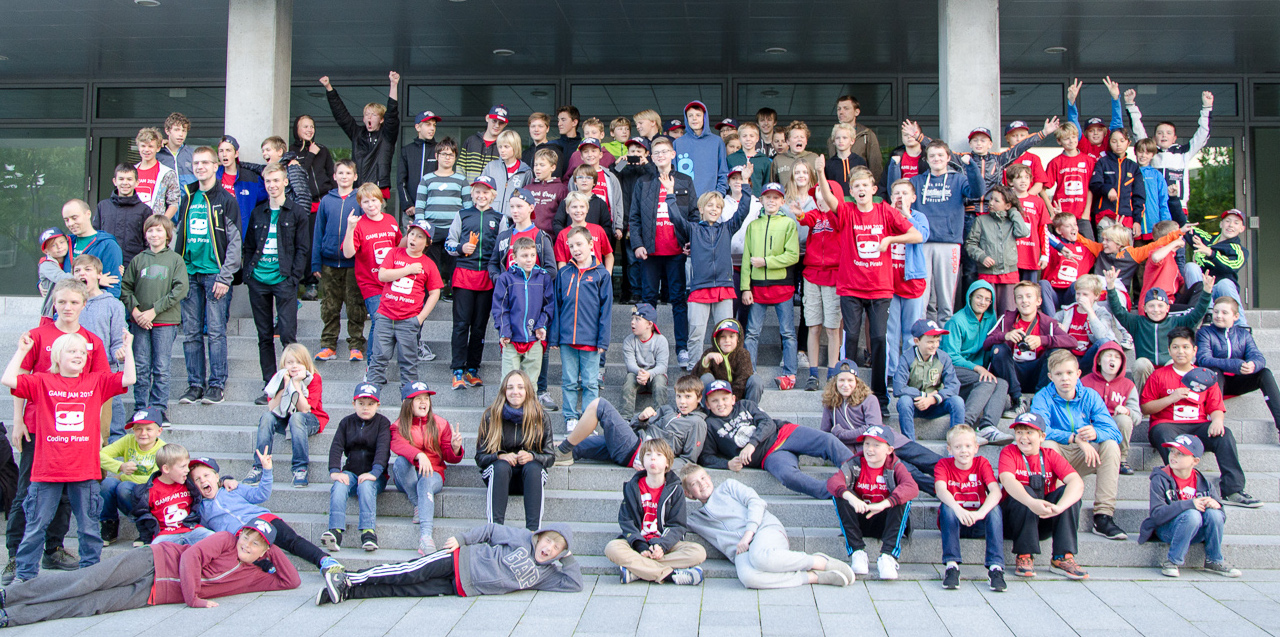
\includegraphics[width=0.9\textwidth]{imagery/gamejam}}
\end{frame}

\begin{frame}
  \frametitle{Partners}

\begin{itemize}
\item Center for Teaching Development and Digital Media, Aarhus
  University
\item Department of Computer Science, University of Copenhagen
\item The libraries
\item Microsoft
\item Computerworld
\item The Danish IT Industri Association
  \begin{itemize}
  \item Canon
  \item CapGemini
  \item NNIT
  \item \ldots
  \end{itemize}
\end{itemize}
\end{frame}

\subsection{Motivation}

\begin{frame}
\frametitle{Motivation}

\begin{textblock}{16}(0,2)
{
\setlength{\fboxsep}{0pt}%
\setlength{\fboxrule}{1pt}%
\only<2>{\centerline{\fbox{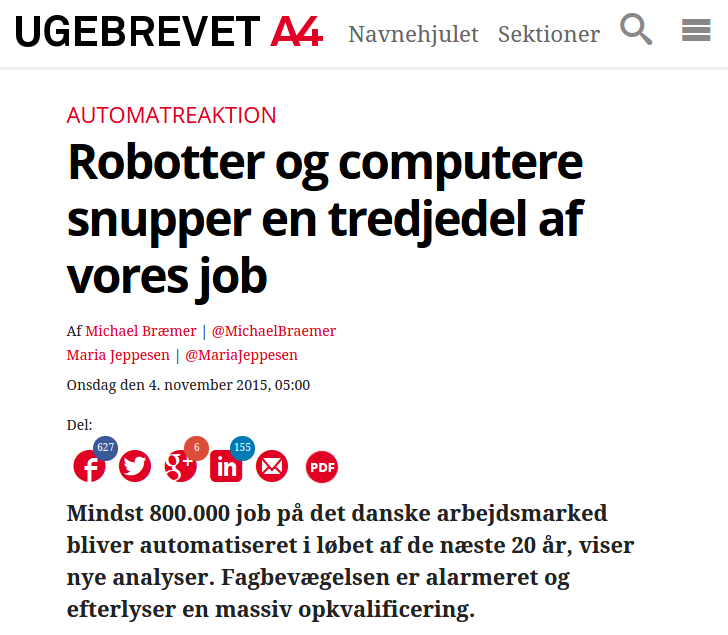
\includegraphics[width=0.5\textwidth]{imagery/ugebreveta4-automatisering}}}}
\only<4>{\centerline{\fbox{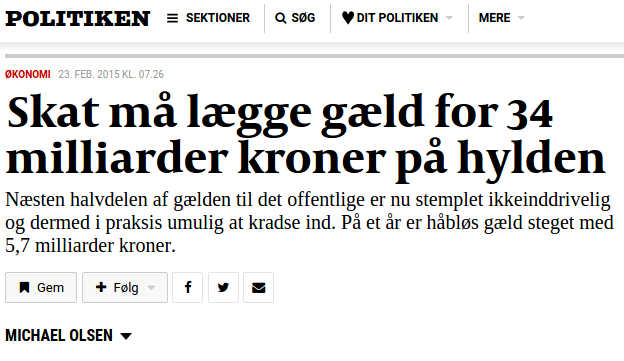
\includegraphics[width=0.5\textwidth]{imagery/skat-efi}}}}
\only<6>{\centerline{\fbox{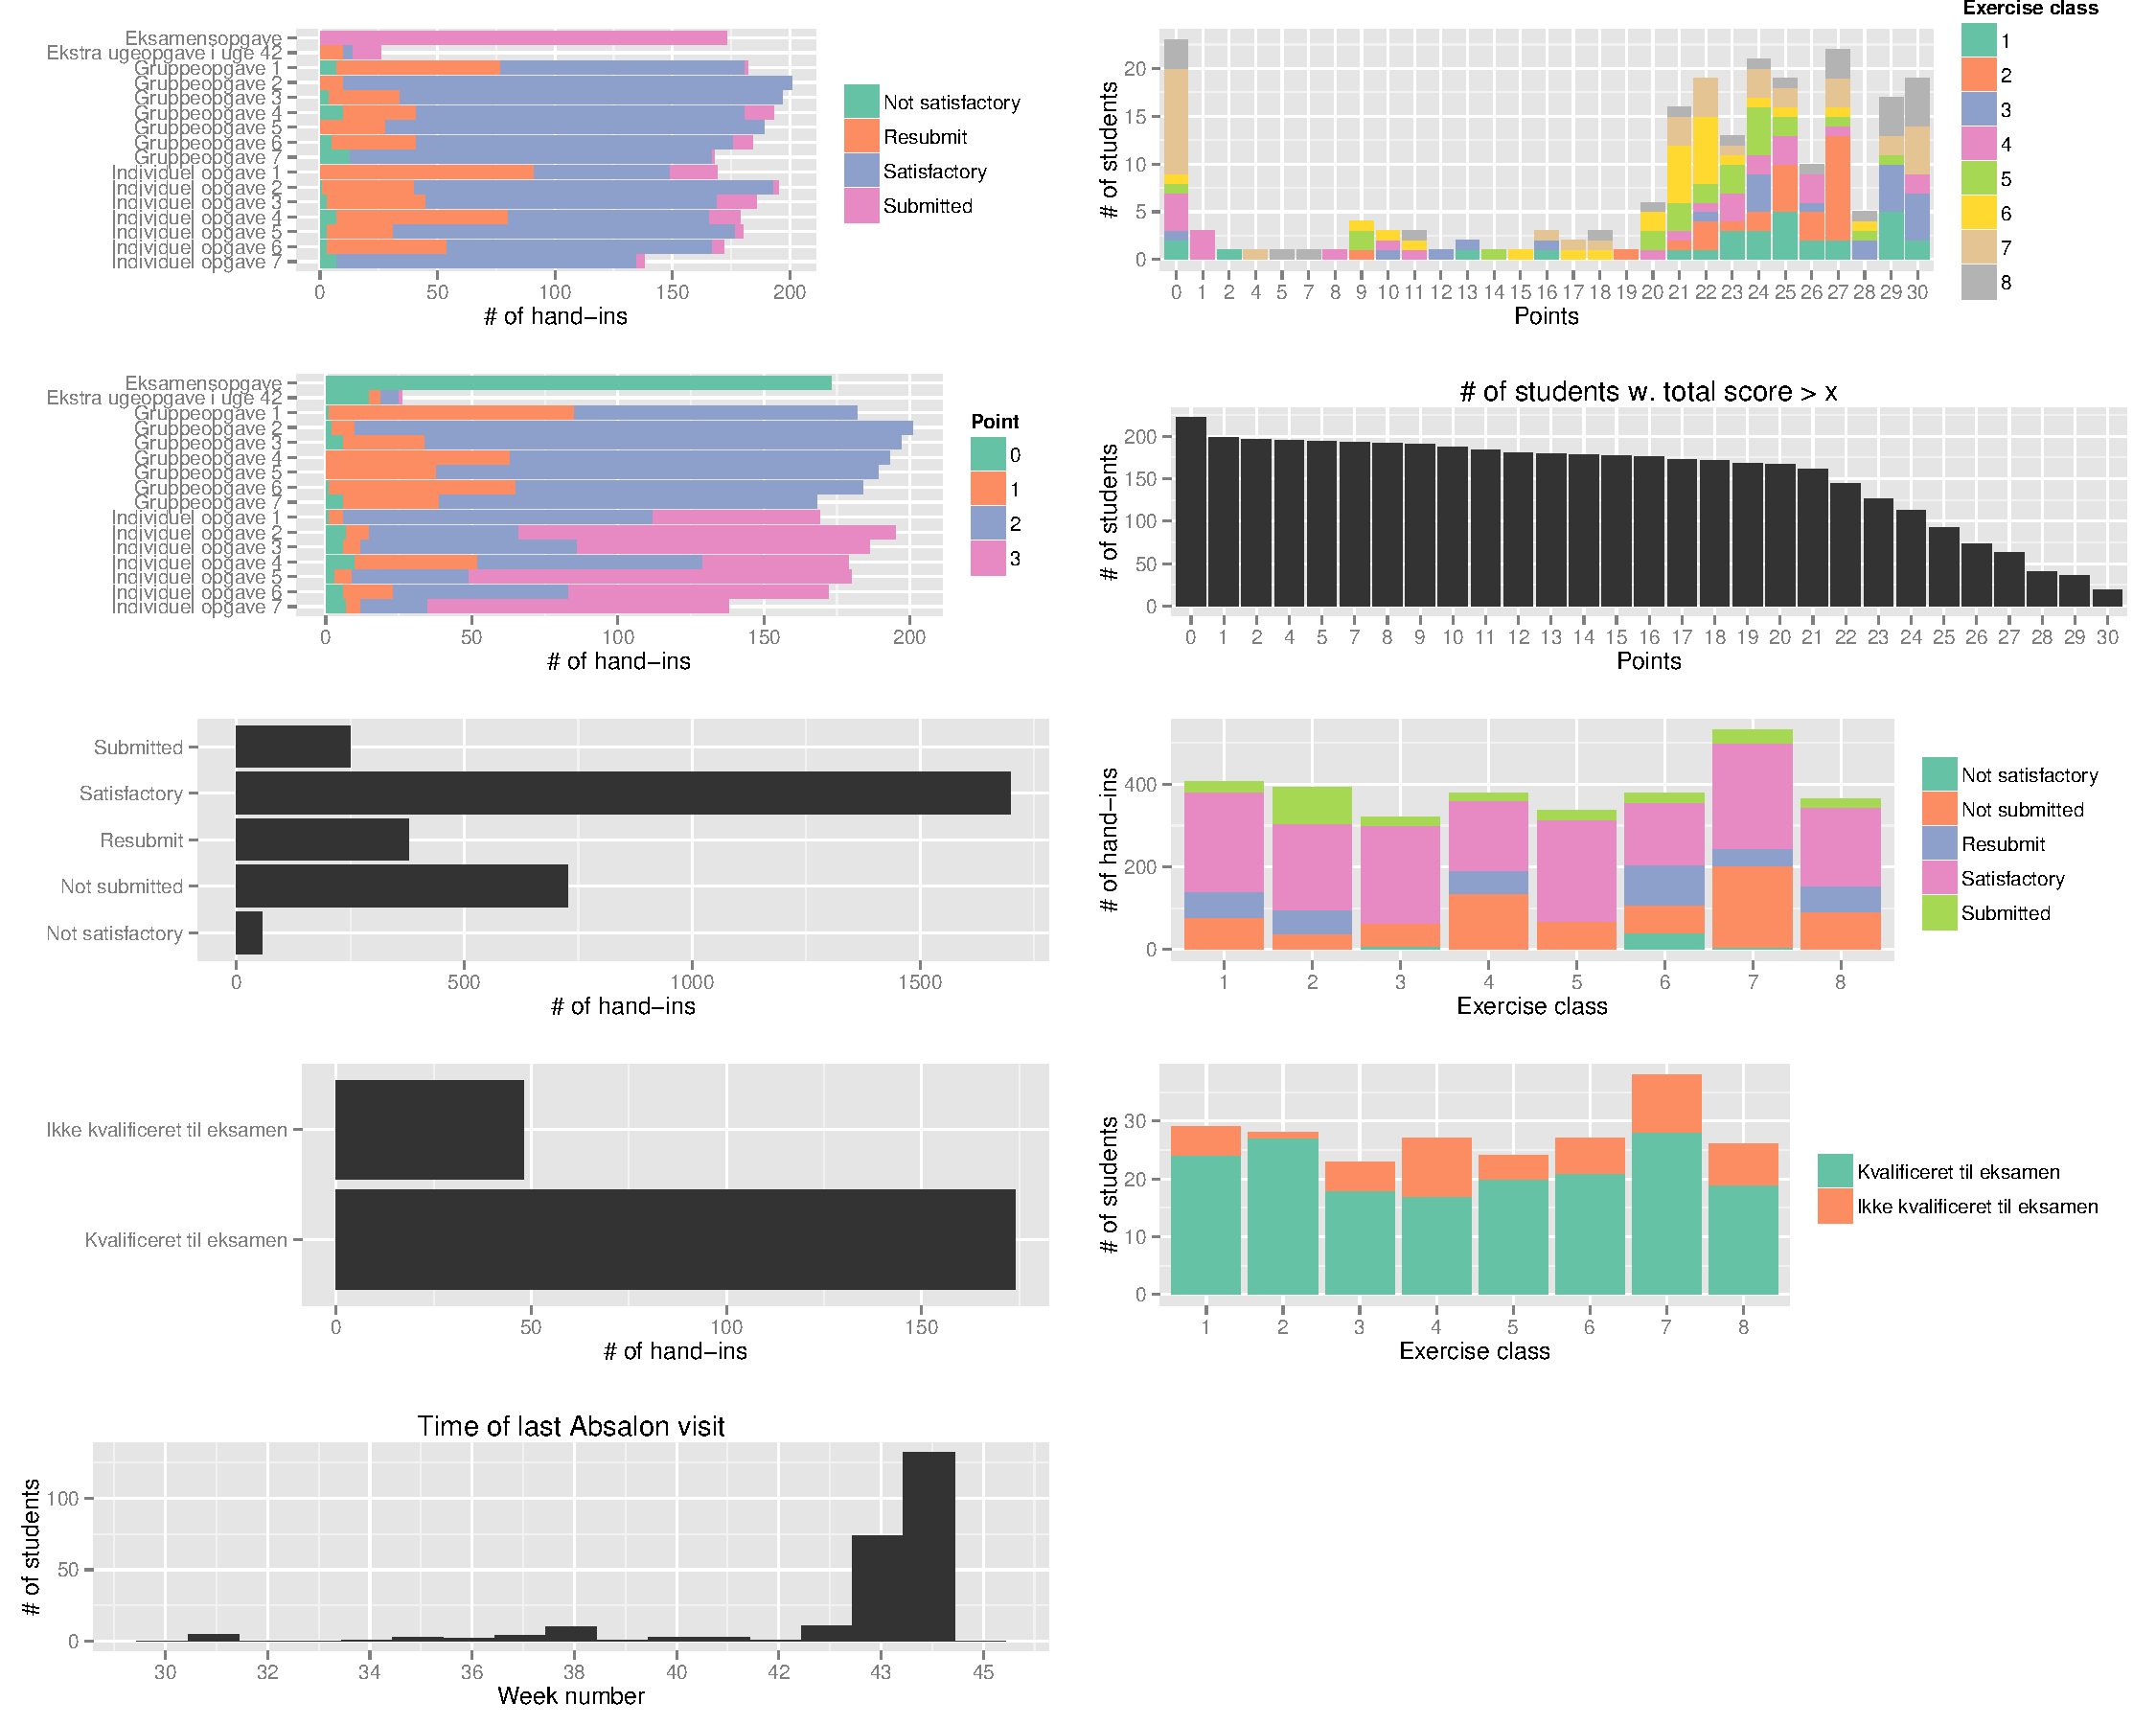
\includegraphics[width=0.7\textwidth]{imagery/ip_allplots}}}}
\only<7>{\centerline{\fbox{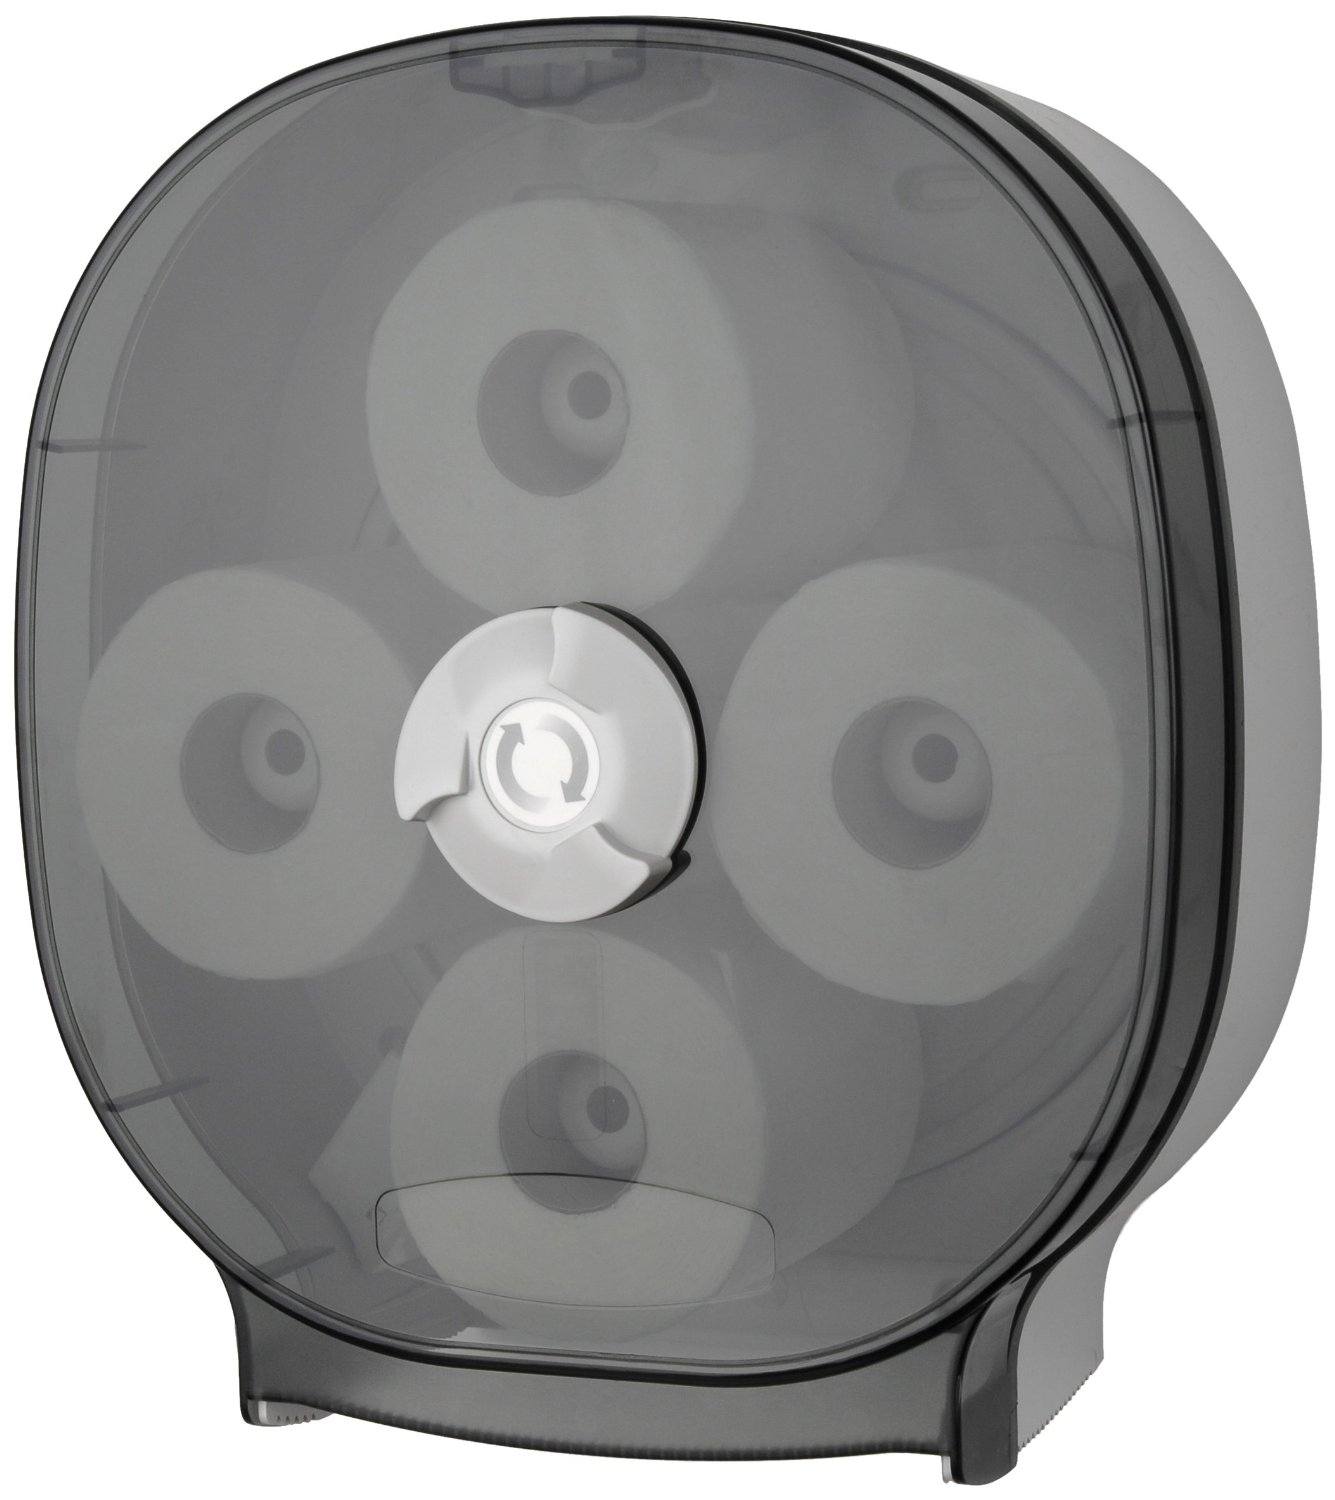
\includegraphics[width=0.5\textwidth]{imagery/toiletpaper-carousel}}}}
}
\end{textblock}

\only<1-7>{
\begin{itemize}
\item Digital revolution, Information Age.
\item Democracy: New tech requires new policies. The public
  should be able to make informed decisions
\item Automatisation
\item Big IT projects $=>$ big problems! Decision makers needs an upgrade
\item Computational thinking is useful everywhere!
\item Because it's 2015!
\end{itemize}
}\end{frame}


\subsection{The Coding Pirates philosophy}
\begin{frame}
\frametitle{The Coding Pirates philosophy}

\begin{itemize}
\item Inspiration from Maker-movement
\item Design thinking
\item Curiosity, exploration
\item Courage, Zest
\item Computational thinking
\end{itemize}

Manifesto: \url{http://codingpirates.dk/manifesto/}

\vspace{5mm}
\begin{quotation}
  "The problems now faced by mankind are largely due to man's own
  creativeness. Creativeness will need to account for much more if
  present problems are to be transcended with solutions".

  - Preface of "Explorations in Creativity", Editors: Ross L. Mooney,
  Taher A. Razik
\end{quotation}
\end{frame}

\begin{frame}
  \frametitle{Example project: Horror teddy bear}
  by Penelope, 12 years
  \vspace{7mm}

  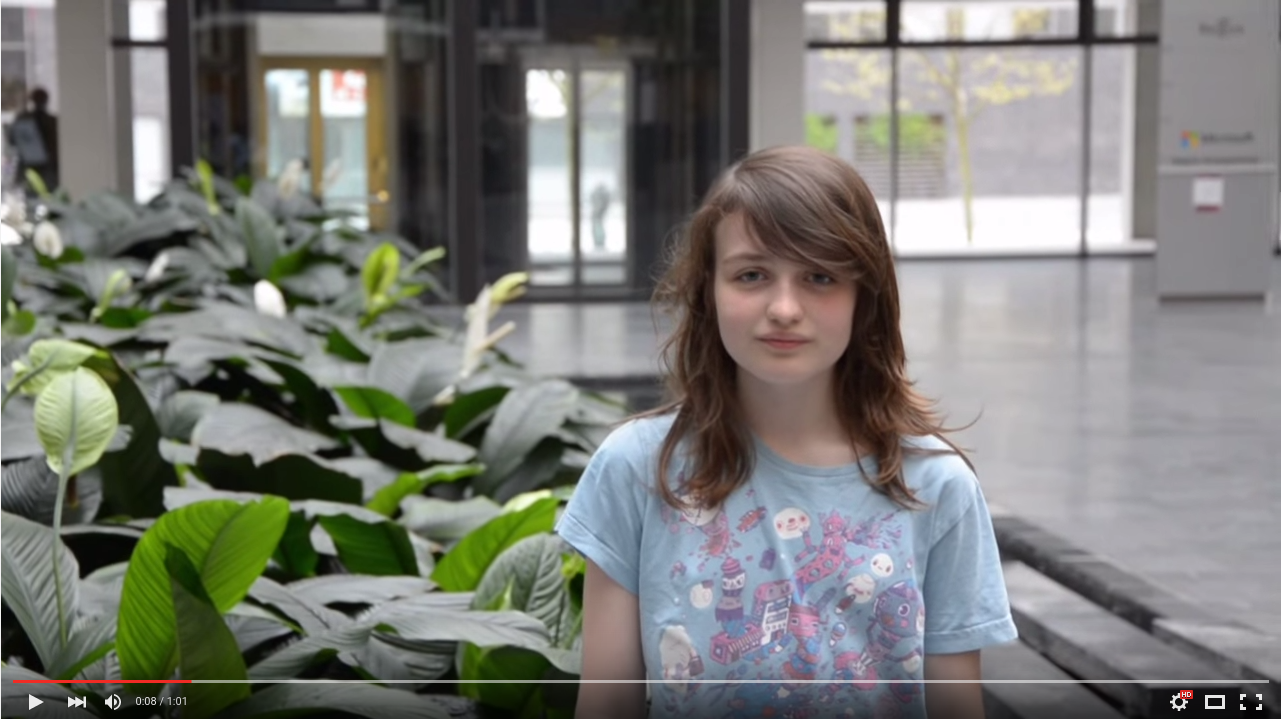
\includegraphics[width=\textwidth]{imagery/penelope-raedselsbamse}

  \url{https://www.youtube.com/watch?v=Mc21BbiUGxU}
\end{frame}



\section{Coding Pirates in practice}
\begin{frame}
\frametitle{In practice}

\begin{textblock}{20}(8,0.5)
 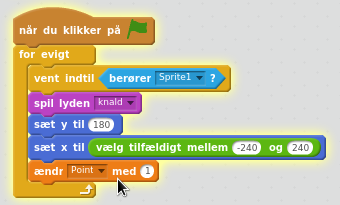
\includegraphics[width=0.3\textwidth]{imagery/scratch}
\end{textblock}

\begin{textblock}{20}(6,9)
  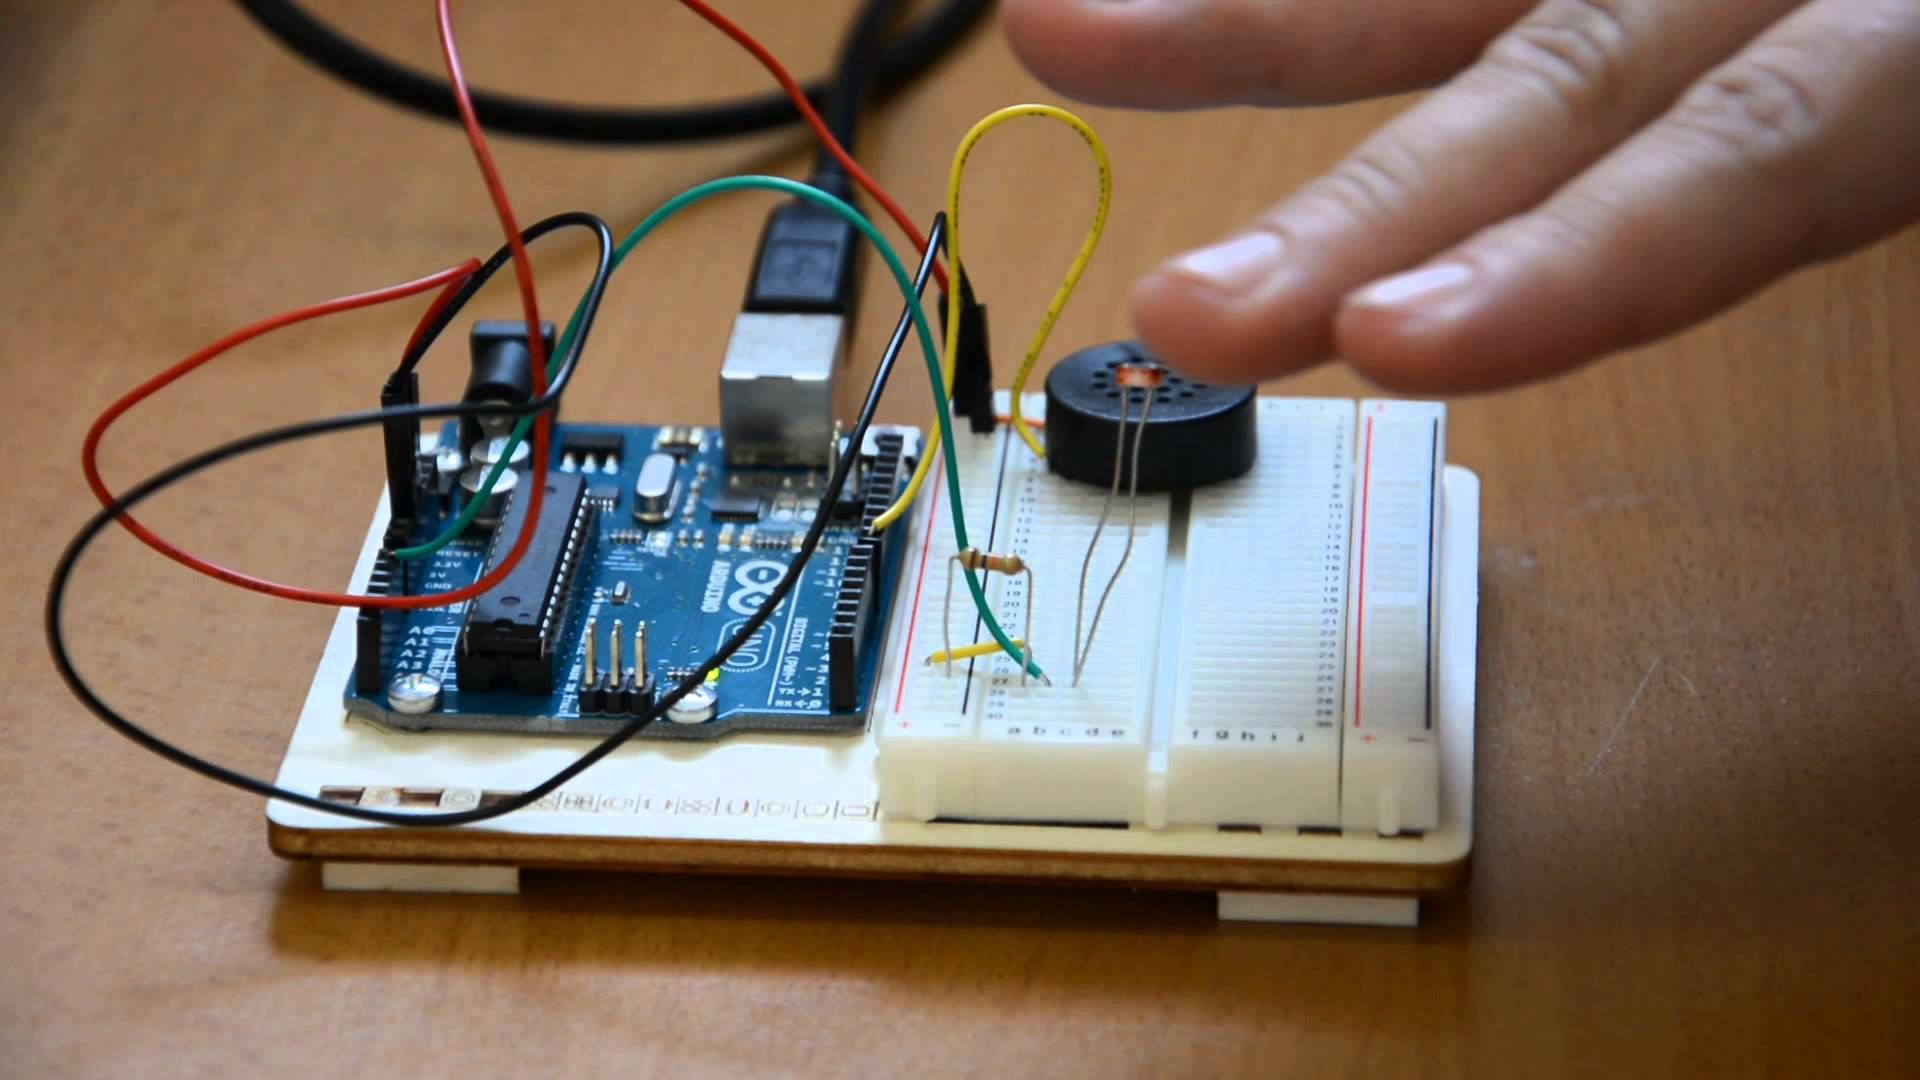
\includegraphics[width=0.4\textwidth]{imagery/arduino-theremin}
\end{textblock}

\begin{itemize}
\item $\sim$25-30 kids
\item $\sim$7-10 volunteers
\item 2 hours a week, usually 17:00-19:00
\item 15 minutes break with snacks, cool aid, fruit etc.
\item Bring your own device (BYOD)
\end{itemize}
\vspace{2cm}

\end{frame}

\begin{frame}
\frametitle{Workshops}

\begin{itemize}
\item 4-6 week workshops
  \begin{itemize}
  \item Scratch
  \item Processing(.js)
  \item Arduino
  \item Unity
  \item Python
  \item 3D modelling in Blender
  \end{itemize}
\item Kids can not switch between workshops during these 4-6 weeks
\item Presentations at the end of a 4-6 week period
\end{itemize}


\end{frame}

\begin{frame}
 \vspace{5mm}
 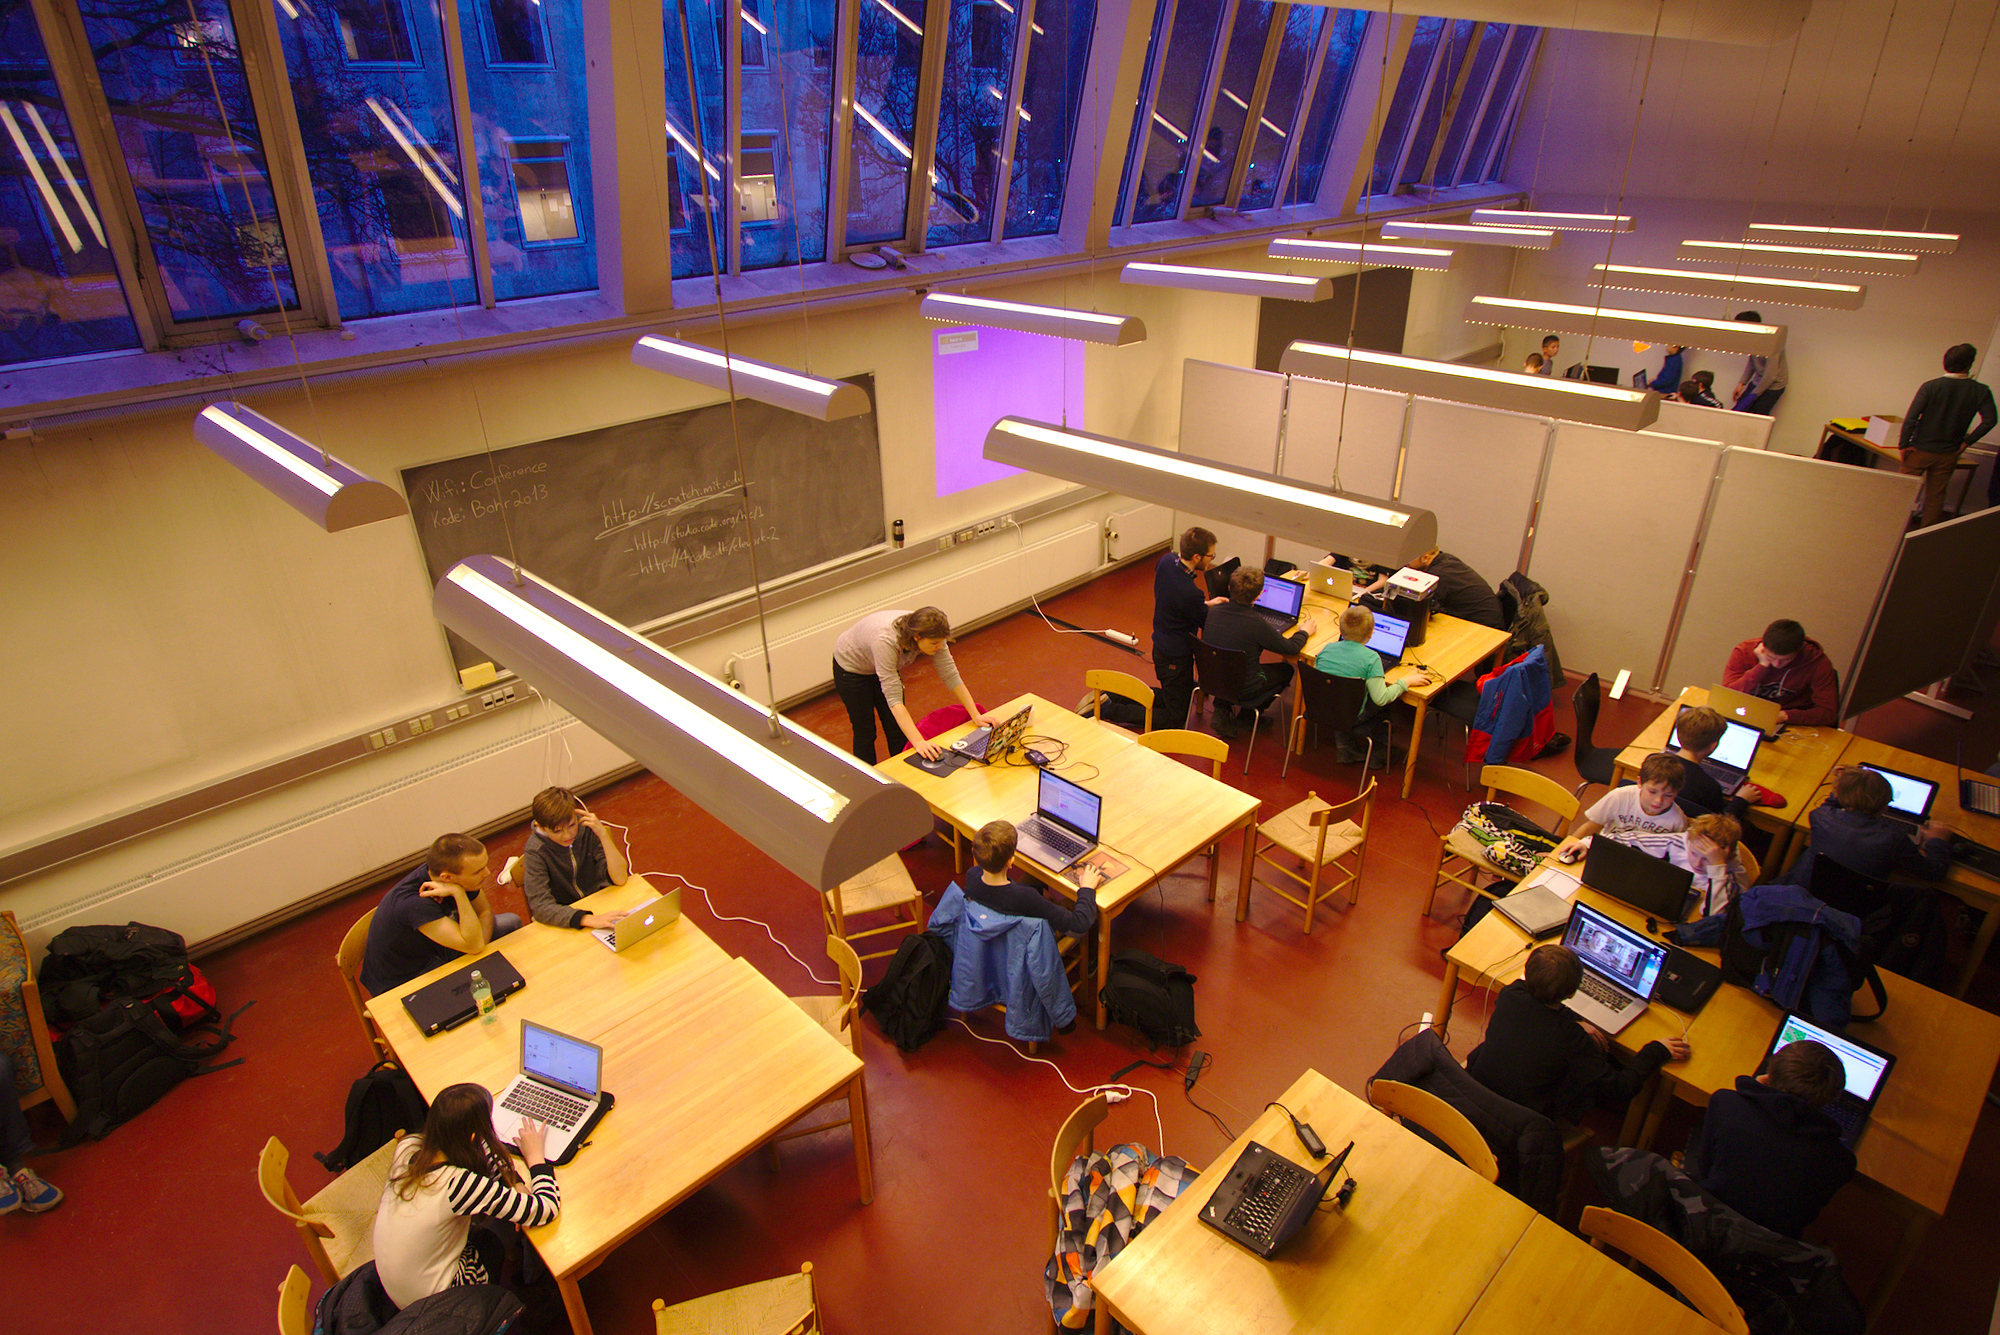
\includegraphics[width=\textwidth]{imagery/codingpirates-diku}
\end{frame}

\begin{frame}
 \vspace{5mm}
 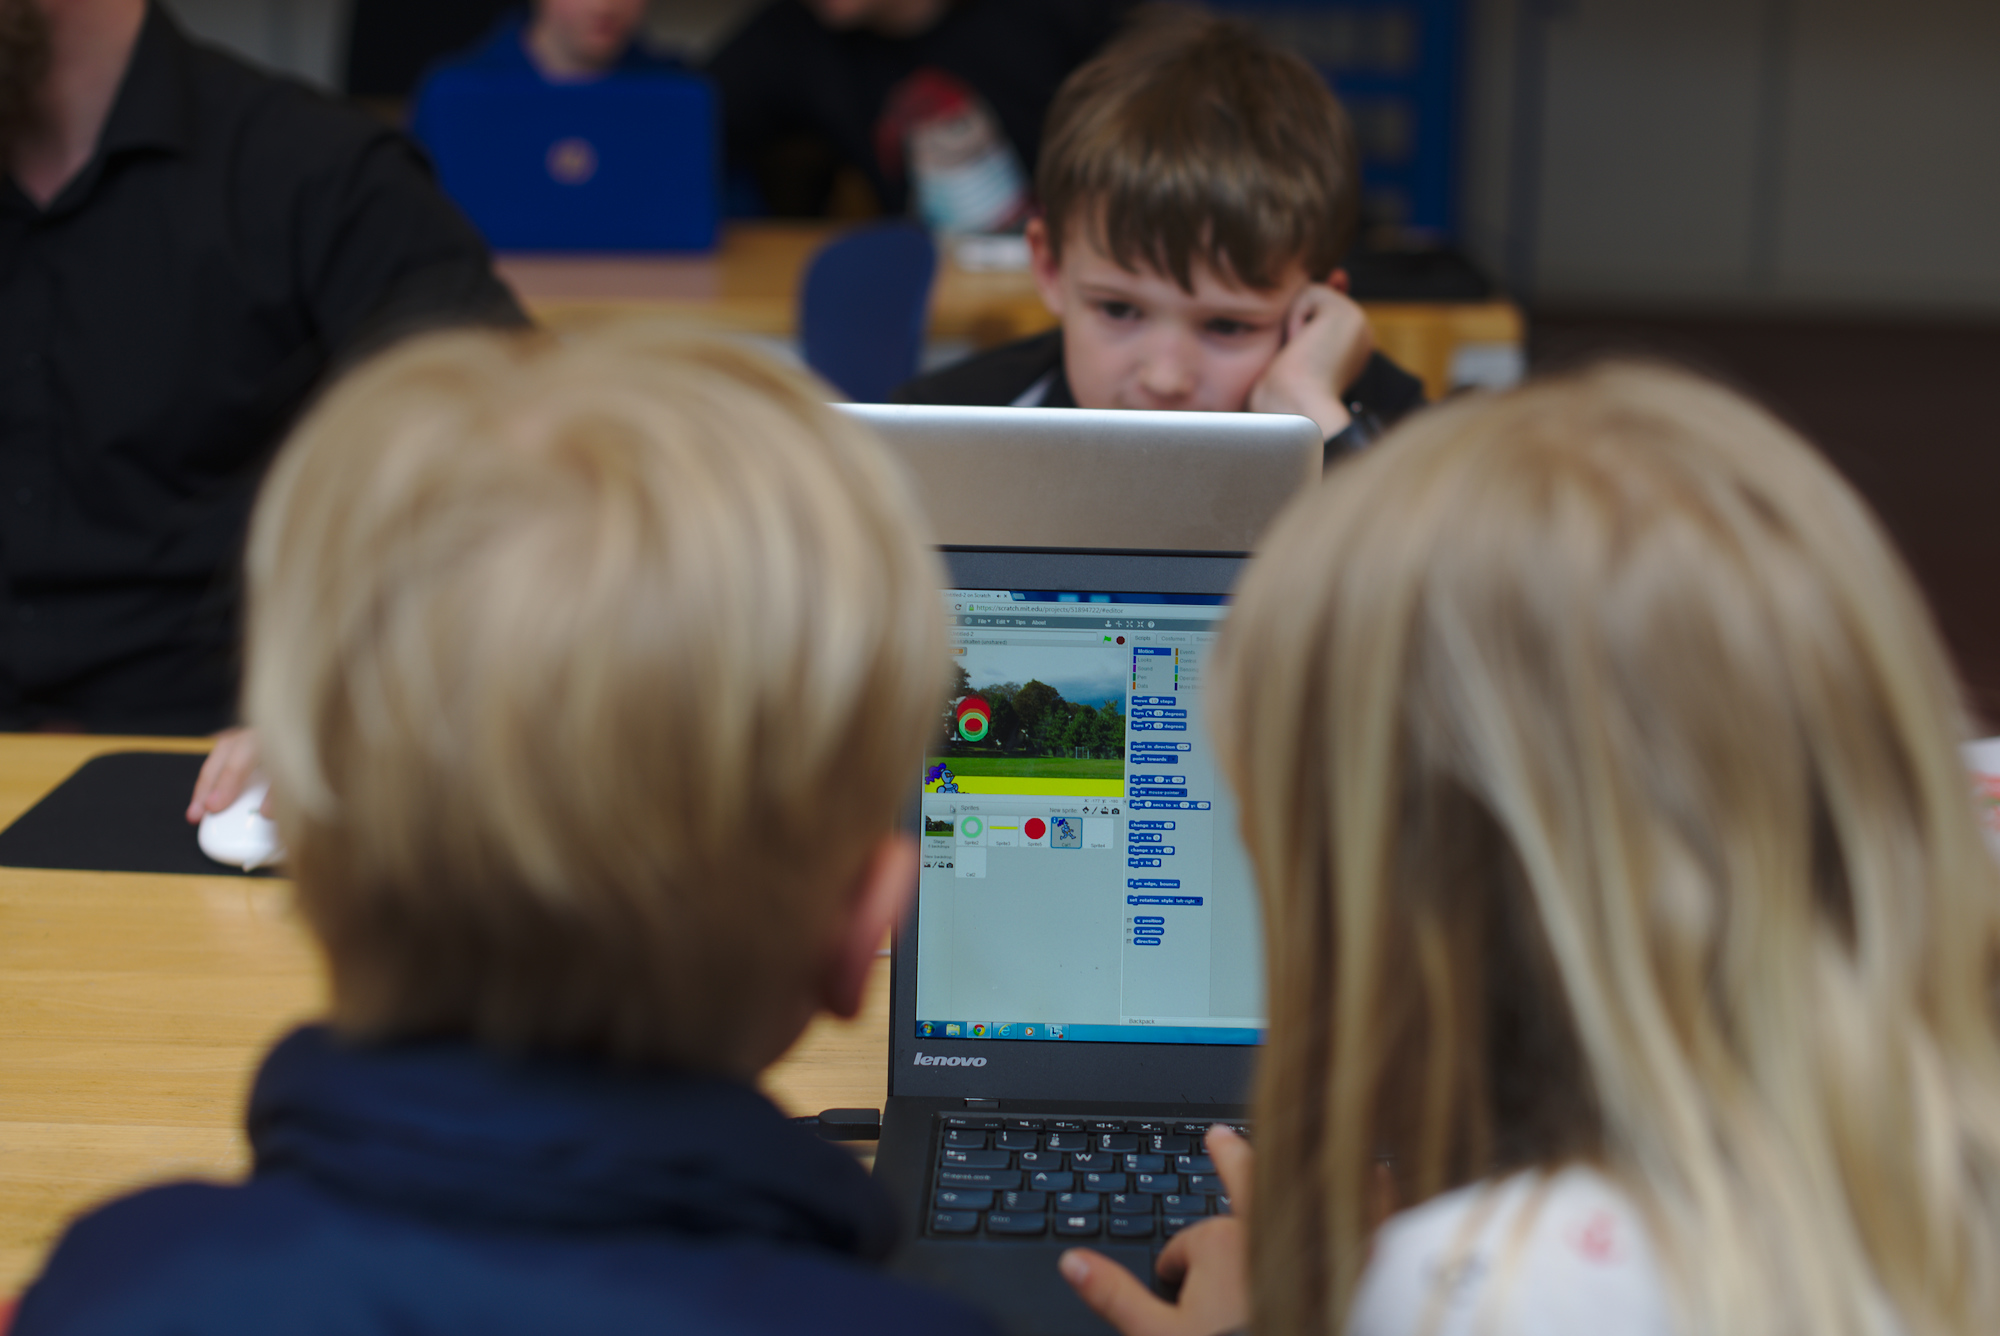
\includegraphics[width=\textwidth]{imagery/william-sofie}
\end{frame}

\begin{frame}
 \vspace{5mm}
 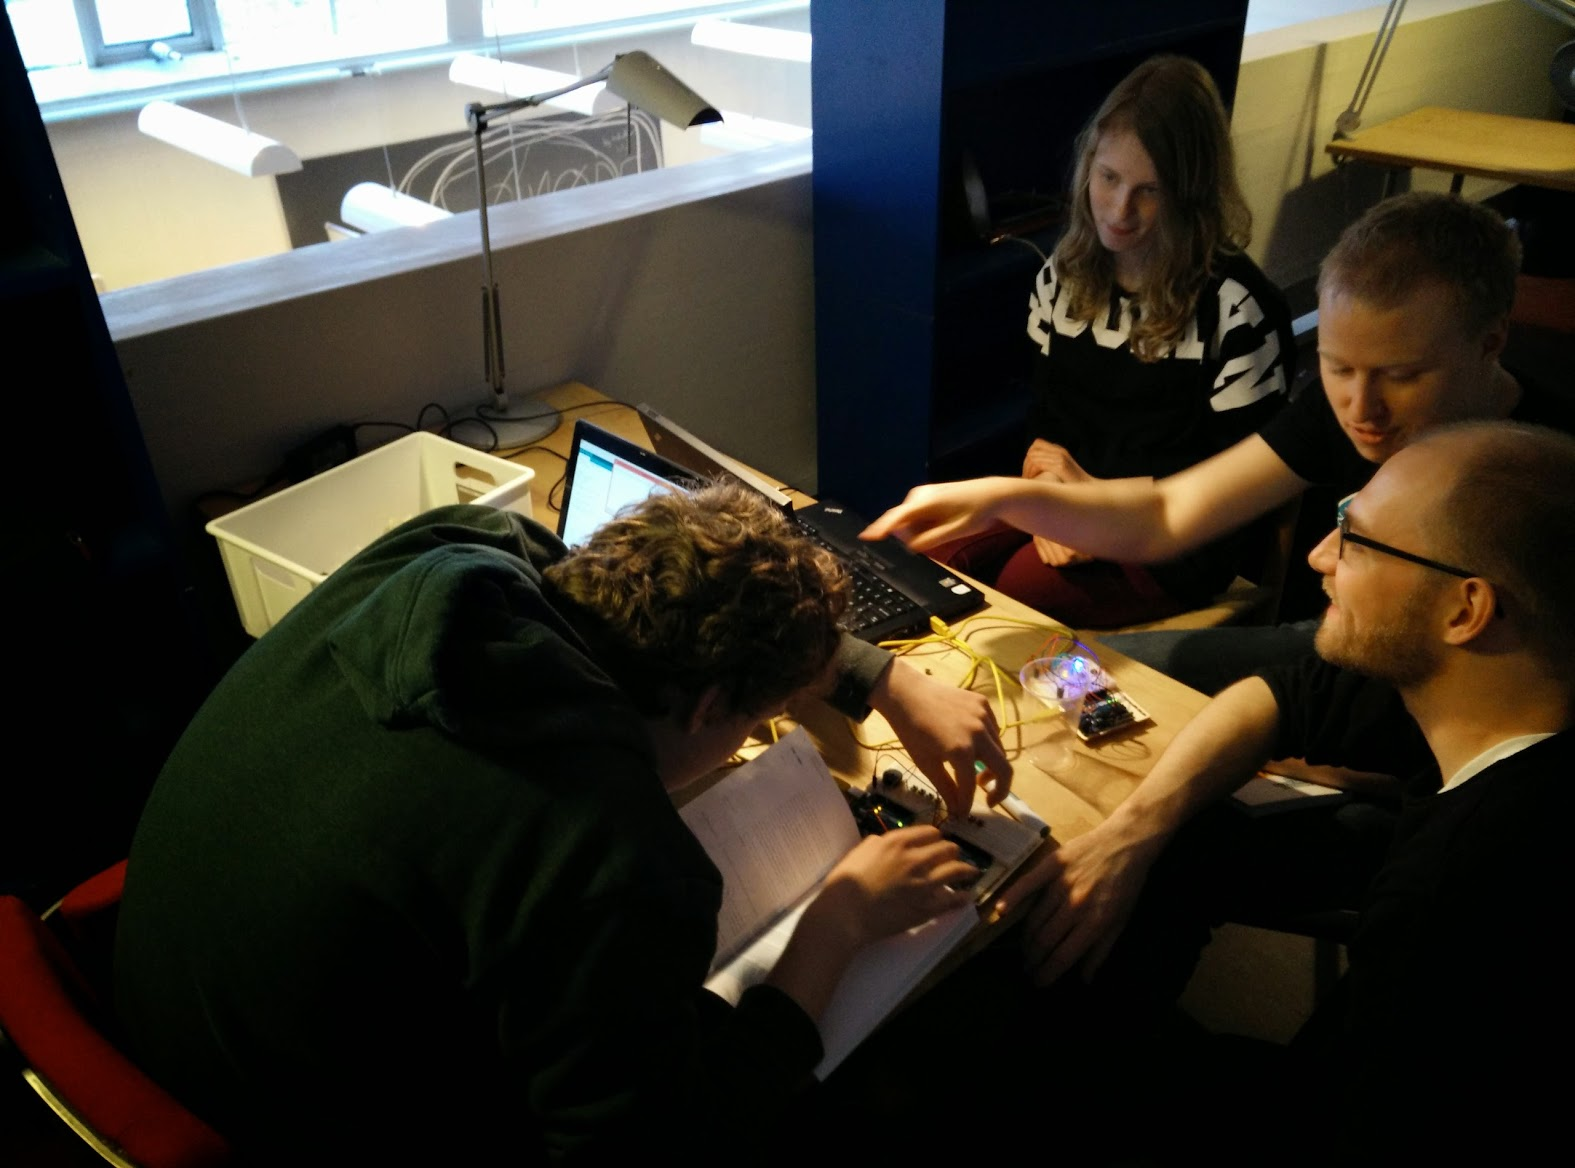
\includegraphics[width=\textwidth]{imagery/arduino-workshop}
\end{frame}

\begin{frame}
 \vspace{5mm}
 \includegraphics[width=\textwidth]{imagery/august-mindstorms}
\end{frame}

\begin{frame}
 \vspace{5mm}
 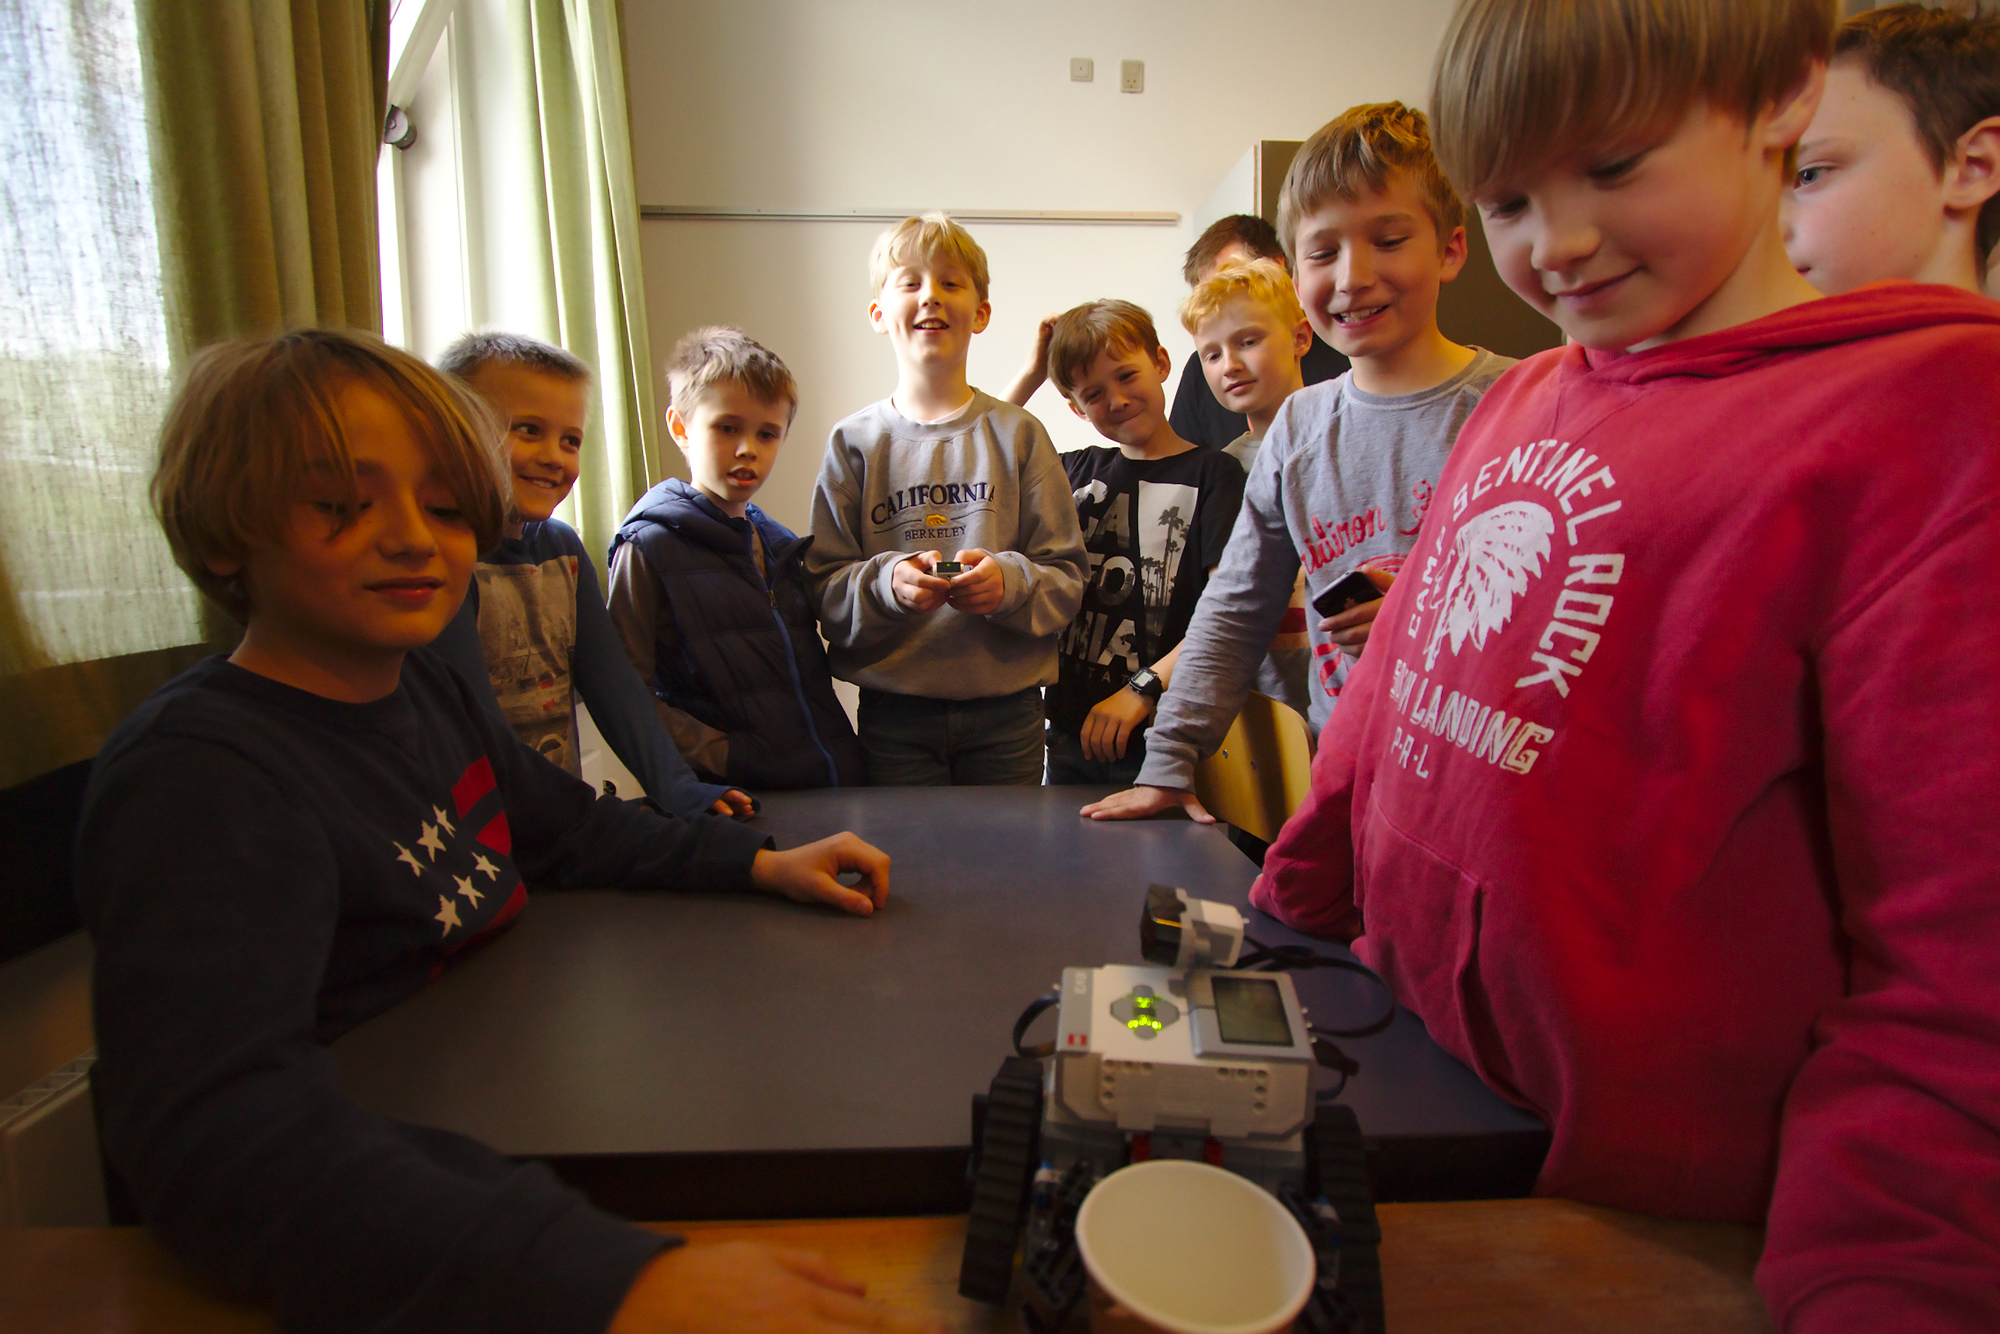
\includegraphics[width=\textwidth]{imagery/mindstorms-presentation}
\end{frame}




\subsection{Scratch}
\begin{frame}
\vspace{1cm}
 
\includegraphics[width=\textwidth]{imagery/scratch-logo}

\end{frame}

% \begin{frame}
% \frametitle{Scratch 4 Arduino}

% \end{frame}

% \section{Processing(.js)}
% \begin{frame}
% \frametitle{Processing(.js)}

% \end{frame}

% \subsection{... and other technologies}
% \begin{frame}

% \frametitle{Other technologies used}
% \todo{find logos}

% \begin{itemize}
% \item Processing(.js) via KhanAcademy
% \item Arduino
% \item Blender (3D modelling)
% \item Unity (2D and 3D games)
% \item LEGO Mindstorms and LEGO WeDo (expensive)
% \item littleBits (expensive)
% \end{itemize}
% \end{frame}

\subsection{Showcase of projects}

\begin{frame}
  \frametitle{Stickman dungeon}
  by Alexander and Oscar, 11 years

  \centerline{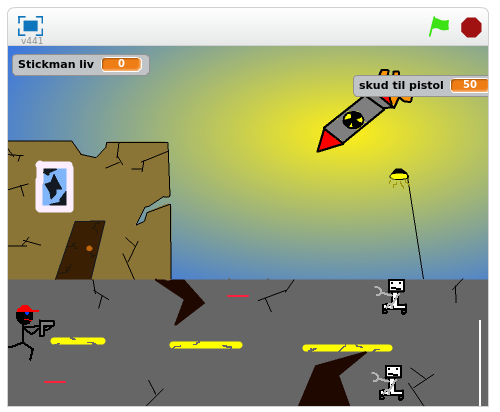
\includegraphics[width=0.8\textwidth]{imagery/stickman-dungeon}}

  \url{https://scratch.mit.edu/projects/57201286/}
\end{frame}

\begin{frame}
  \frametitle{Robot-sumo}
  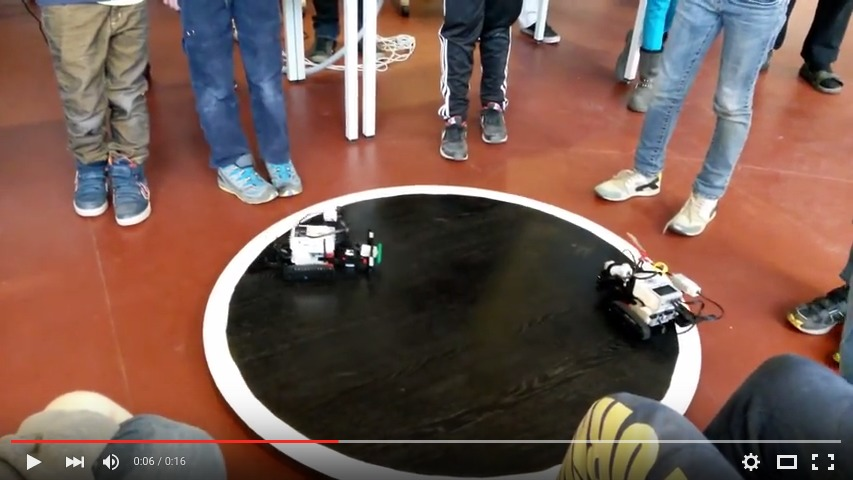
\includegraphics[width=\textwidth]{imagery/robotsumo}
  
  \url{https://www.youtube.com/watch?v=qcWTpXh-rOw}
\end{frame}


\begin{frame}
  \frametitle{3D printed autonomous Arduino boat}
  by Niels, 12 years

  \vspace{2mm}
  \centerline{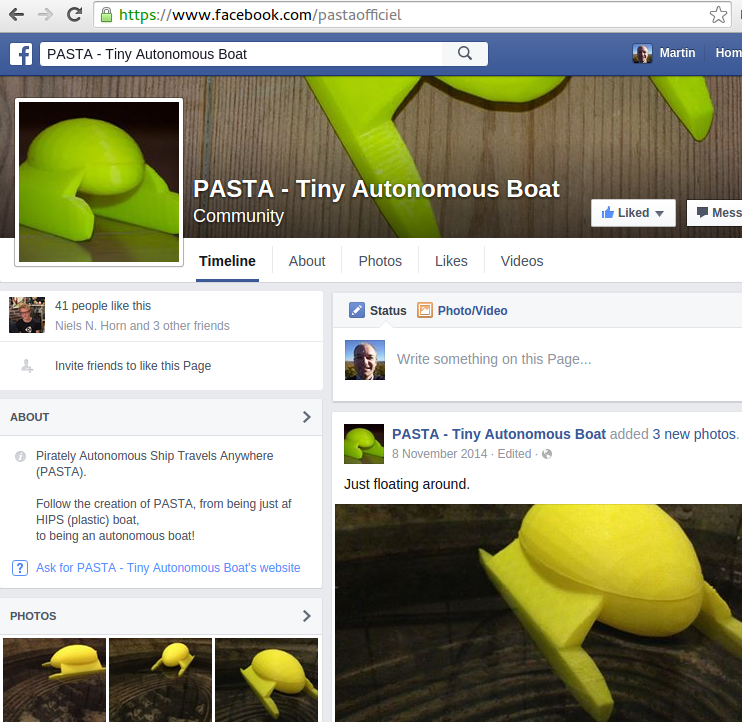
\includegraphics[width=0.8\textwidth]{imagery/pasta_autonomous_submarine}}
\end{frame}

\begin{frame}
  \frametitle{iOS app: ``Draw the wall''}
  by William, 14 years

  \vspace{2mm}
  \centerline{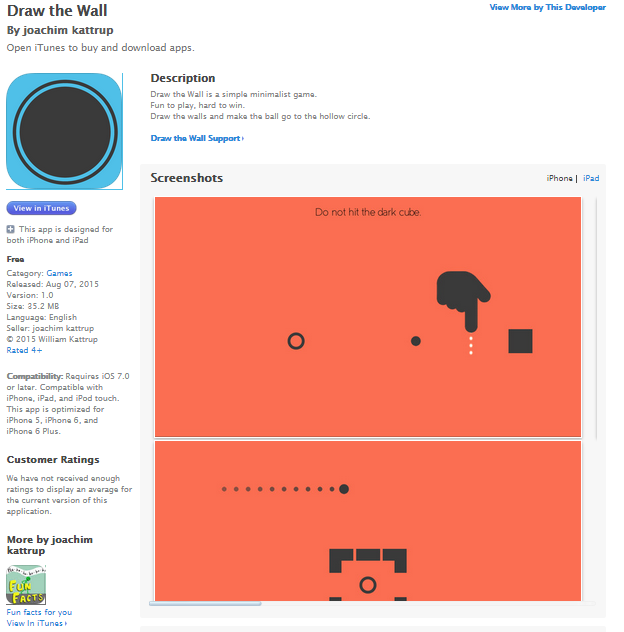
\includegraphics[width=0.8\textwidth]{imagery/drawthewall}}
\end{frame}



\subsection{Difficulties ahead}
\begin{frame}
\frametitle{Difficulties}
\begin{itemize}
\item Few from age 14 and up
\item Few girls
\item Fostering friendships is hard, but important
  \begin{itemize}
  \item Force pair programming?
  \end{itemize}
\item Further education of volunteers
\end{itemize}
\end{frame}

\begin{frame}
  \frametitle{Age and gender (including waiting list)}
  \centerline{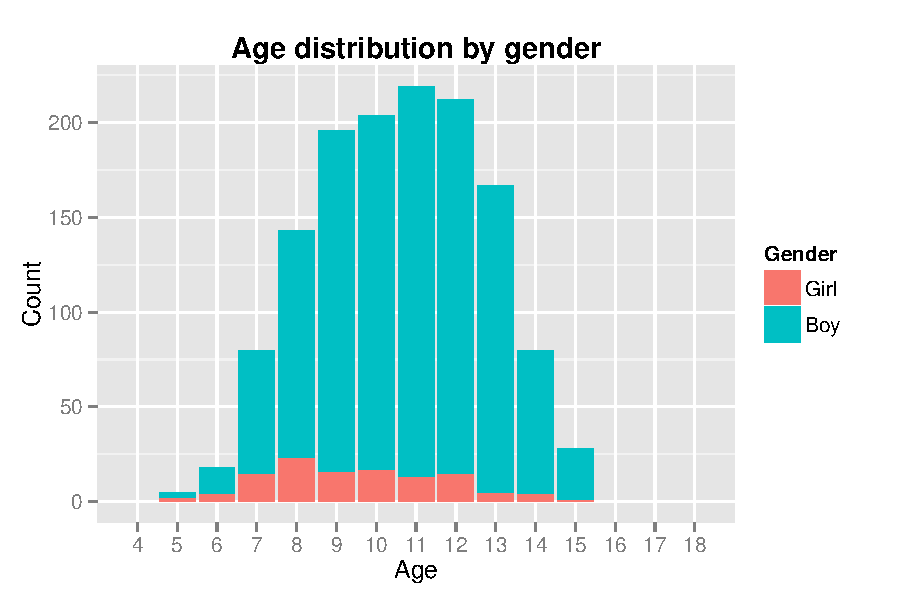
\includegraphics[width=\textwidth]{../datacrunching/age-gender-hist}}
\end{frame}

\begin{frame}
  \frametitle{Percentage of girls by age (including waiting list)}
  \centerline{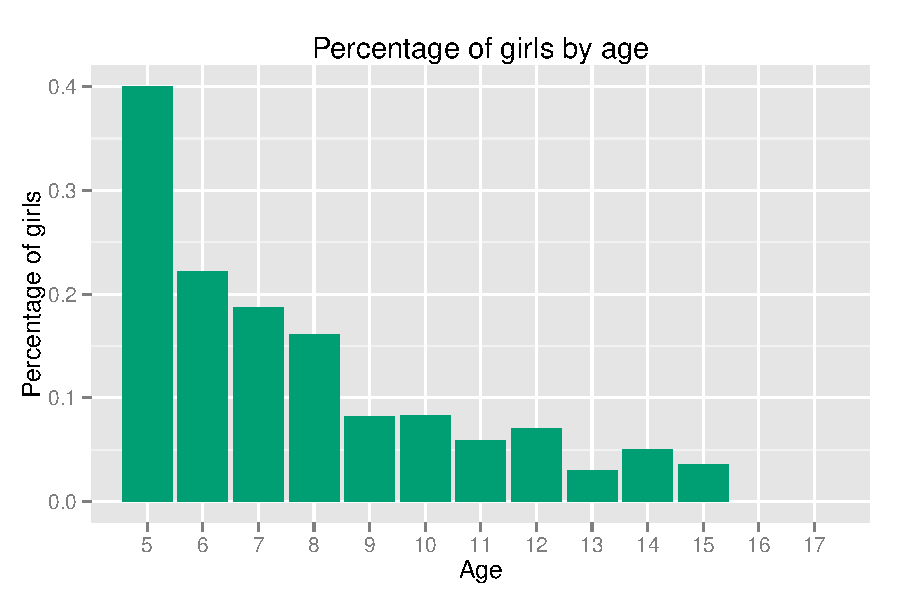
\includegraphics[width=\textwidth]{../datacrunching/girl_percentage}}
\end{frame}

\subsection{The Coding Pirates Community}
\begin{frame}
  \frametitle{Volunteer community}
  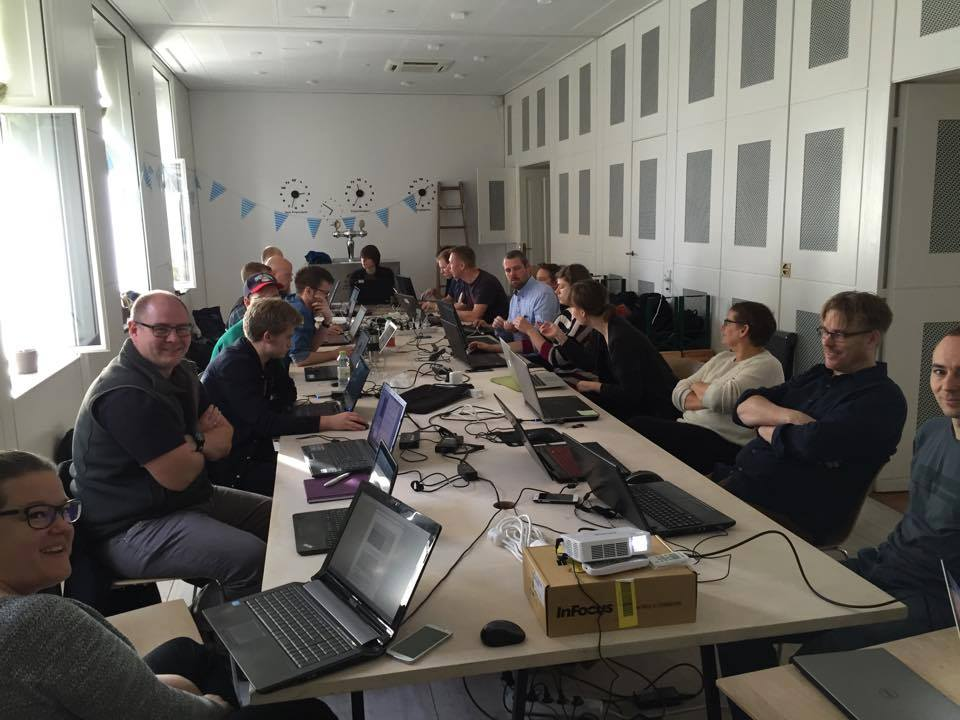
\includegraphics[width=\textwidth]{imagery/unity-for-volunteers.jpg}
\end{frame}


\section{Computing in schools}
\begin{frame}
  \frametitle{Computing in schools}
  \begin{quotation}
    "The computer is the Proteus of machines. Its essence is its
    universality, its power to simulate. Because it can take on a
    thousand forms and can serve a thousand functions, it can appeal
    to a thousand tastes."

    - Seymour Papert, in Mindstorms
  \end{quotation}

  We can already use this when teaching e.g. history, biology, chemistry,
  or language classes!

  \begin{itemize}
  \item Make a game that teaches grade $N-1$ about photosynthesis
  \item Make a game that teaches grade $N-1$ about life in ancient Rome
  \item Make an interactive story that tells the story XYZ
  \end{itemize}

  More fun than a poster or a written report!
\end{frame}

\begin{frame}
  \frametitle{But what do we want schools to teach?}

  \begin{itemize}
  \item Teach computing as a discipline, e.g. like math
    \begin{itemize}
    \item Algorithms vs. data
    \item Systematic problem solving
    \item Computational thinking
    \end{itemize}
  \item Teach computing as a craft/skill, e.g. like woodwork
    \begin{itemize}
    \item Focus on creation and tools
    \item Creative and reflective thinking
    \end{itemize}
  \item A mix?
  \item As a separate discipline or inside other classes?
  \end{itemize}
\end{frame}

\section{DIKU's involvement}
\begin{frame}
\frametitle{Why does a university use time teaching tweens and teens?}
\begin{itemize}
\item Supply chain management
\item The teachers needs our expertise
\item Defining how computing should be taught in Schools
\item Potential research areas
\item Teacher education and re-education
\item Because we have connections to potential volunteers (e.g. alumni)
\item Good publicity and great advertisement
\end{itemize}
\end{frame}

\begin{frame}
  \centerline{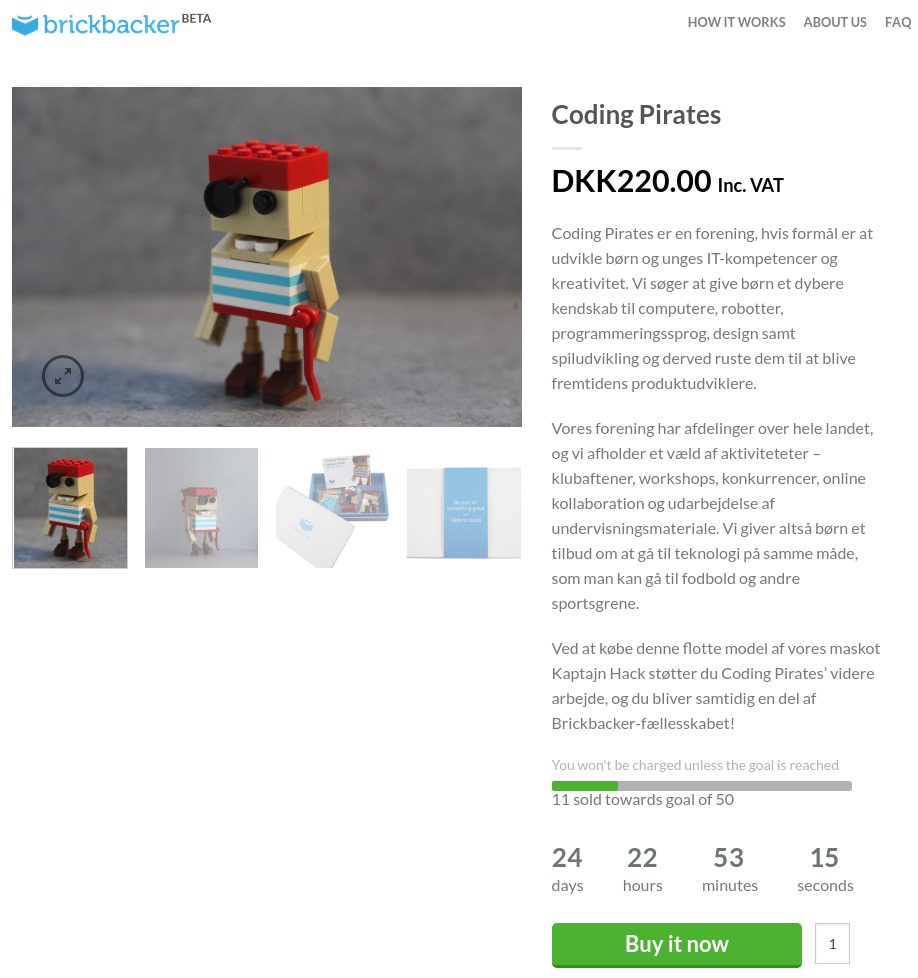
\includegraphics[width=\textwidth]{imagery/brickbacker}}
\end{frame}


\begin{frame}
  \frametitle{Coding Pirates in Gothenburg?}
  \begin{center}
    
\includegraphics[origin=c,angle=-20,width=0.7\textwidth]{imagery/wanted}
  \end{center}

\end{frame}

\begin{frame}
  \frametitle{Links}
  \begin{itemize}
  \item Website: http://codingpirates.dk
  \item Facebook: https://www.facebook.com/codingpirates
  \item Manifesto: http://codingpirates.dk/manifesto/
  \item Scratch labyrinth: https://scratch.mit.edu/projects/55351416/
  \item Brickbacker: http://brickbacker.com/product/codingpirates/
  \item DigiPippi: http://digipippi.dk
  \end{itemize}
\end{frame}


\end{document}